\newpage
%%%%%%%%%%%%%%
\section{Dise\~ no}
%%%%%%%%%%%%%%
\begin{comment}
\textit{Debe describir el dise\' ~o y su implementaci\' on. Se deben incluir diagramas de bloques o de estados, en caso de ser necesario. Deben explicar c\' omo funciona el dise\' ~o, y tener claro qu\' e elementos son clave de mencionar para que el lector pueda comprender c\' omo funciona el dise\' ~o. No incluya simulaciones en esta secci\' on, no incluya informaci\' on detallada del c\' odigo Verilog, la explicaci\' on debe ser de alto nivel. Debe brindarse una discusi\' on balanceada entre lo que usted implement\' o y porqu\' e se eligi\' o esa implementaci\' on. }
\end{comment}

\subsection{Generalidades}


La figura \ref{fig:DiagramaInicial} muestra el diseño inicial para el procesador de 5 etapas de pipelining con todas las especificaciones dadas.

\begin{figure}[H]
	\centering
		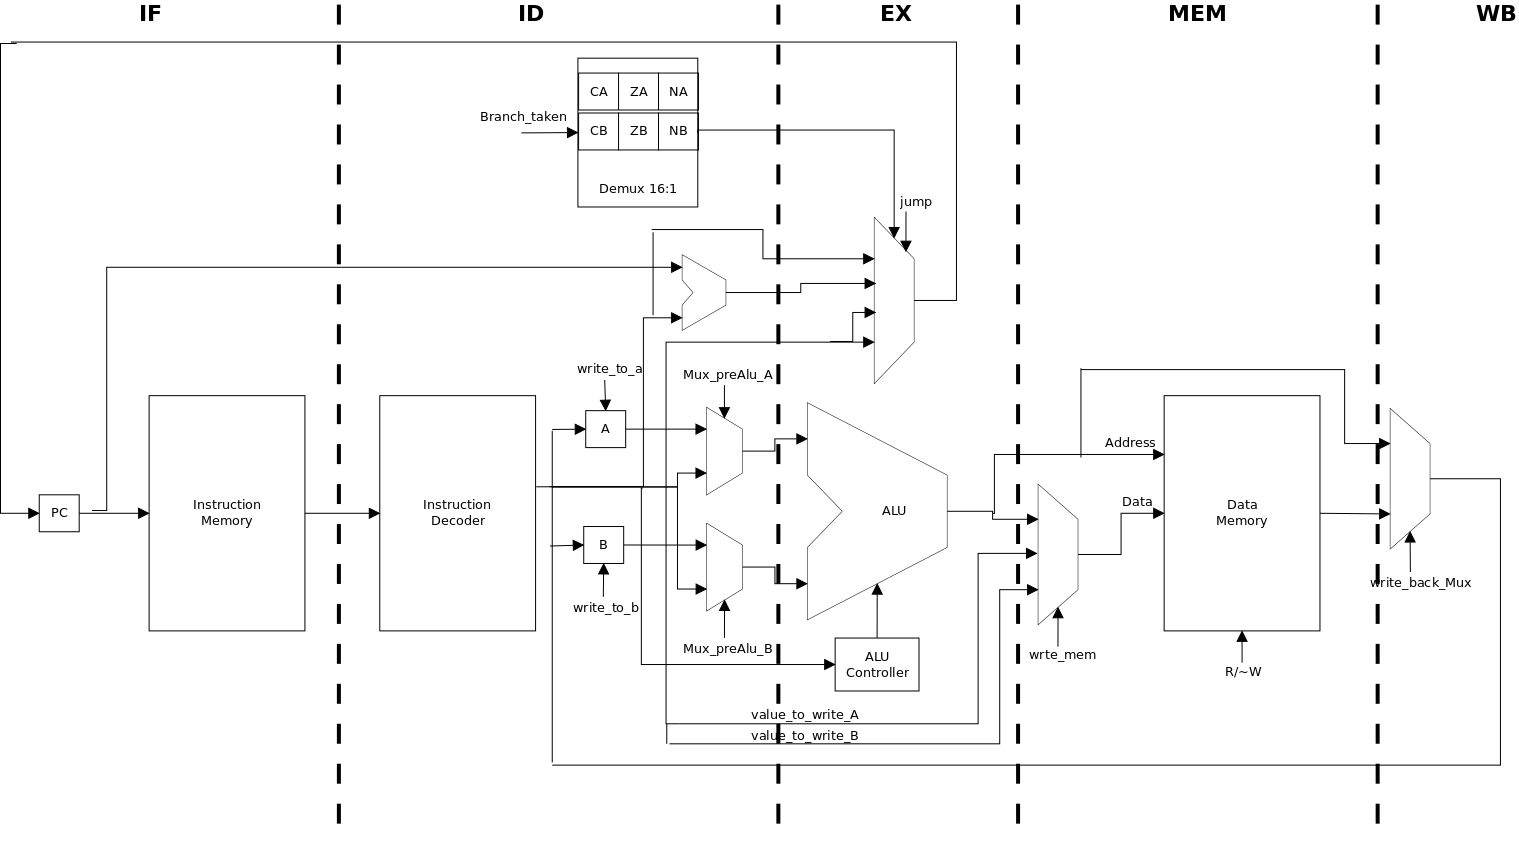
\includegraphics[width=\textwidth]{./imagenes/DiagramaInicial}
	\caption{Diagrama inicial que ejemplifica el diseño}
	\label{fig:DiagramaInicial}
\end{figure}

A continuación se va a explicar la función de cada uno de los bloques, dividido en cada una de las etapas del pipelining.

\subsection{Etapa Instruction Fetch (IF)}

En esta etapa se obtiene de la memoria de instrucciones la instrucción que se va a procesar en ese siguiente ciclo.

\subsubsection{Módulo PC}

El módulo PC es un registro sencillo, encargado de almacenar la dirección de memoria de la que se quiere obtener la dirección. Esta, en forma normal, incrementa uno cada ciclo, para apuntar a la siguiente posición de memoria, y leer la instrucción siguiente; sin embargo, con los branches y los jumps, existe una lógica para calcular la nueva dirección.

\subsubsection{Instruction Memory}

Es una memoria asincrónica sencilla, con 1024 posiciones de memoria (10 bits de bus de direcciones) y sus datos son de 16 bits, los cuales, el decodificador los va a interpretar acorde a lo especificado en el enunciado, según sea la instrucción.

\subsection{Etapa Instruction Decoding (ID)}

En esta etapa, principalmente, se decodifica la instrucción recibida, y se configuran todas las señales de control acorde a lo necesitado dependiendo de la instrucción. 

\subsubsection{Instruction Decoder}

Se encarga de decodificar la instrucción y de definir todas las señales de control. Las señales de control manejadas por este módulo son:

\begin{itemize}

\item write\_to\_a y write\_to\_b: Cuando se da llega a la etapa de Write Back (explicada posteriormente), si esta señal está en alto, permite que se realice una escritura en alguno de los dos registros, colocando la señal respectiva en alto.

\item Mux\_preAlu\_A y Mux\_preAlu\_B: Señales de control que manejan los multiplexores colocados previos a la ALU. Estos definen qué dato se ingresa a la ALU, si el proveniente del registro A (o del B, según el caso), o el proveniente directamente del Decoder. Esta elección varía dependiendo del tipo de instrucción que se debe ejecutar. Por ejemplo: para un acceso a memoria, se requiere de una dirección, proveniente directamente del Instruction Decoder; en cambio, para una suma, se necesita del dato contenido en A o en B.

\item Branch\_taken: Esta señal se encarga de comunicarle al Demux qué tipo de branch es el que se quiere evaluar, y dependiendo del que sea, se analiza el bit de status correspondiente. 

\item jump: Esta señal se coloca en alto únicamente en los casos en que la instrucción que se debe ejecutar sea un JMP (Jump). Esto coloca al sistema en un modo en el que se puede modificar el contador del programa a un nuevo valor, definido por la instrucción leída.

\item write\_mem: Esta señal define cual dato es el que se quiere ingresar en la memoria de datos: si el dato contenido en A, en B, o el proveniente de la ALU. Esto se utiliza para los casos en que se realiza un Store.

\item R/\~W: Esta señal controla si la memoria de datos está en modo de lectura o de escritura.

\item write\_back\_mux: Define si el dato que se escribe de vuelta en los registros es el proveniente de la ALU o de la memoria de Datos.
\end{itemize}

\subsubsection{Registros A y B}

Funcionan como Acumuladores. Son registros que almacenan los datos provenientes de la etapa de Write Back. Se controlan por las señales write\_to\_a y write\_to\_b, respectivamente, como se explicó anteriormente.


\subsubsection{Módulo de cálculo de branch}

Este módulo se encarga del cálculo del nuevo valor del contador de programa, en caso de que el branch sea tomado finalmente. Este módulo consiste en una suma del contador de programa actual, con el valor indicado en la instrucción que se quiere desplazar relativamente ya sea hacia arriba o hacia abajo, dependiendo del valor del sétimo bit.

\subsubsection{Módulo de branch taken}

Este módulo se encarga de definir si el branch es tomado o no, dependiendo de los 6 bits de status que se tienen especificados: $C_A$, $Z_A$, $N_A$, $C_B$, $Z_B$, y $N_B$. Dependiendo del tipo de instrucción que sea, se referencia alguno de los bits de status y se define si el branch se toma o no.
%%
Adem\' as se encarga de efectuar el c\' alculo del nuevo PC, por lo que debe ser capaz de tomar en cuenta el tipo de instrucci\' on que esta ejecut\' andose, y el valor de las banderas antes mencionadas. Se trata de usar una se\~ nal de control que elija en un mux 4:1, donde las entradas son PC+1, Branch Magnitude, JMP direcci\' on, JMP direcci\' on.


\subsection{Etapa de Ejecución (EX)}

Se realiza el cálculo necesario según sea la instrucción especificada. Las diferentes operaciones se realizan en la ALU.

\subsubsection{M\' odulo de controlador de ALU}
Este es el m\' odulo del procesador que se encarga de manejar todas las se\~ nales de control que se utilizan para controlar la unidad l\' ogico arim\' etica. Su funci\' on principal se puede resumir en que debe ser capaz de determinar la operaci\' on que se debe efectuar a partir de los 6 bits m\' as significativos de la instrucci\' on decodificada, por lo tanto tiene una entrada de 6 bits y una salida de 3 bits.


\subsubsection{M\' odulo ALU}

Este es el m\' odulo del procesador que se encarga de efecuar los c\' alculos aritm\' eticos y la ejecuci\' on del \textit{pipeline} de manera que se cumpla con la etapa (EX). En t\' erminos generales es un m\' odulo que recibe dos entradas de 10bits cada una y tiene una salida de 10bits y una entrada de se\~ nal de control proveniente del m\' odulo controlador de alu de acuerdo a como se puede observar en la tabla \ref{tab:alu_operands}. Cualquier operaci\' on que no est\' a presente en la tabla se asigna con el valor de $\$ 7$ en cual es usado para decir que la alu no debe realizar ninguna operaci\' on con los operandos, lo cual es as\' i para todos los saltos condicionales e incondicionales, as\' i como tambien para la \textbf{NOP}. 

% Please add the following required packages to your document preamble:
% \usepackage[normalem]{ulem}
% \useunder{\uline}{\ul}{}

\begin{table}[h]
\begin{tabular}{cccccc}
\multicolumn{6}{c}{{\bf \ul Controlador de ALU, valores en octal}}                                                                                               \\
{\bf Instrucci\' on} & {\bf C\' odigo} & \multicolumn{1}{l|}{{\bf Decodificado}} & {\bf Instrucci\' on} & {\bf C\' odigo} & {\bf Decodificado} \\
LDA                  & 0               & \multicolumn{1}{l|}{0}                  & SUBA                 & 12              & 3                  \\
LDB                  & 1               & \multicolumn{1}{l|}{0}                  & SUBB                 & 13              & 3                  \\
LDCA                 & 2               & \multicolumn{1}{l|}{0}                  & SUBCA                & 14              & 3                  \\
LDCB                 & 3               & \multicolumn{1}{l|}{0}                  & SUBCB                & 15              & 3                  \\
STA                  & 4               & \multicolumn{1}{l|}{0}                  & ANDA                 & 16              & 2                  \\
STB                  & 5               & \multicolumn{1}{l|}{0}                  & ANDB                 & 17              & 2                  \\
ADDA                 & 6               & \multicolumn{1}{l|}{1}                  & ANDCA                & 20              & 2                  \\
ADDB                 & 7               & \multicolumn{1}{l|}{1}                  & ANDCB                & 21              & 2                  \\
ADDCA                & 10              & \multicolumn{1}{l|}{1}                  & ORA                  & 22              & 5                  \\
ADDCB                & 11              & \multicolumn{1}{l|}{1}                  & ORB                  & 23              & 5                  \\
ASLA                 & 26              & \multicolumn{1}{l|}{4}                  & ORCA                 & 24              & 5                  \\
ASRA                 & 27              & \multicolumn{1}{l|}{6}                  & ORCB                 & 25              & 5                 
\end{tabular}
\caption{Esta tabla muestra la codificaci\' on del controlador de ALU para las instrucciones en las que se debe realizar una operaci\' on}
\label{tab:alu_operands}
\end{table}





\subsection{Etapa de Almacenamiento en Memoria (MEM)}
La etapa de MEM es en la cual se realiza la escritura de datos en la memoria principal de datos, se puede observar que cuando se ocupa realizar una instruccion de escribir desde los registros hasta la memoria, los datos se almacena en el registro EX/MEM, luego para el siguiente ciclo de reloj, los datos se transportan hacia la memoria. 

De igual manera la direcci\' on de memoria calculada por la ALU se almacena en el registro EX/MEM y se ingresa a la memoria principal para el siguiente ciclo de reloj. As\' i como tambien cuando toca almacenar resultados de operaciones aritm\' eticas desde la ALU hasta la memoria de datos.

La \' unica ocaci\' on en que la etapa EX/MEM no utiliza la memoria principal es cuando se realiza una instrucci\' on de salto, o cuando se debe almacenar un dato en uno de los registros en lugar de la memoria principal.




\subsection{Etapa de Write Back (WB)}
La etapa del procesador que se encarga de escribir desde los registros hasta la memoria principal o de la ALU hacia los registros deben pasar por esta etapa por lo tanto cuenta con ciertas se\~ nales de control como se puede observar en el diagrama arquitect\' onico.

Para esta etapa realmente la duraci\' on del ciclo no esta relacionada con el manejo de la instrucci\' on, sino m\' as bien con la duraci\' on de la memoria principal para las lecturas y escrituras. En este caso  dado que la simualaci\' on es conductual y no presenta retardos de propagaci\' on, no se tiene en cuenta este factor, sin embargo, si es importante hacer la aclaraci\' on de que en un caso real, la mayor parte del tiempo que se encuentre en este ciclo es por acceso de la memoria principal.


